\section{Proof of attack on PoPoW}
\label{sec:attack-full}

We now show that, if the statistical properties of blockchains are not respected
in some execution, our construction presented in the main paper is insecure by
illustrating an explicit attack against our scheme.
% We show that this attack is applicable in the same
% manner against our construction as it is applicable against the previous
% PoPoW work~\cite{popow}. PoPoW serves as the starting point and inspiration for
% our protocol. The security proof is incorrect, and in fact the PoPoW protocol is
% susceptible to a double-spending attack within the model (i.e., that can be
% carried out by an attacker with less than 50\% hash power)
During the
exposition of this attack, a simple patch for our construction, which will also
lead to a correct generic security proof, will become clear.

% We focus on illustrating why the PoPoW construction of previous work is insecure
% against an adversary controlling less than $50\%$ of hashing power. The attack
% immediately carries over to our straw man construction introduced above, a
% vulnerability we will address in later sections.
We proceed in two steps. We
first show that a powerful attacker can break chain superquality with
non-negligible probability. Then we construct a concrete double spending attack
based on this observation assuming an attacker of sufficiently high hashing
power (but still below $50\%$).
% Note that maintaining chain superquality was not
% in the original security model; however, we show how the property affects the
% security of the underlying blockchain proofs.

\subsection{Attacking chain superquality}
\label{subsec:superquality-attack}
We construct an adversary $\mathcal{A}$ that breaks the superchain quality at level $\mu$.
% Suppose $\mathcal{A}$ controls a portion $t/n$ of the hashing power.
$\mathcal{A}$ works as follows. Assume she wants to attack the honest party $B$
in order to have him adopt chain $\chain_B$ which has a bad distribution of
superblocks, i.e. such that local goodness is violated in some sufficiently long
subchain. She continuously determines the current chain $\chain_B$ adopted by
$B$. The adversary starts playing after $|\chain_B| \geq 2$. If
$\emph{level}(\chain_B[-1]) < \mu$, then $\mathcal{A}$ remains idle. However,
if $\emph{level}(\chain_B[-1]) \geq \mu$, then $\mathcal{A}$ attempts to mine
an adversarial block $b$ on top of $\chain_B[-2]$. If successful,  she attempts
to mine another block $b'$ on top of $b$. If successful again, she broadcasts
$b$ and $b'$. The adversarial mining continues until $B$ adopts a new chain,
which can be due to two reasons: Either the adversary successfully mined $b, b'$
on top of $\chain_B[-2]$ and $B$ adopts them; or one of the honest parties mined
a block which was adopted by $B$. In either case, the adversary restarts
the strategy by inspecting $\chain[-1]$ and acting accordingly. An execution of
this attack is illustrated in Figure~\ref{fig.superquality-attack}.

\begin{figure}[h]
    \caption{Superquality attack on prior work (PoPoW)~\cite{popow}.
    The adversary performs a selfish-mining~\cite{selfish} attack (gray blocks)
    whenever any honest parties have recently mined a rare $\mu$-superblock
    (black). The attack reduces the honest chain's superquality, while the
    attacker's private chain is unaffected. }
    \centering
    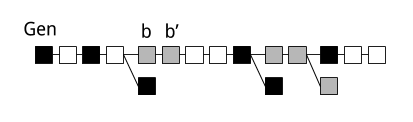
\includegraphics[width=0.5 \columnwidth,keepaspectratio]{chapters/work/figures/superquality-attack-popow.png}
    \label{fig.superquality-attack}
\end{figure}

Assume now that an honestly-generated $\mu$-superblock was adopted by $B$ at
position $\chain_B[i]$ at round $r$. We now examine the probability that
$\chain_B[i]$ will remain a $\mu$-superblock in the long run. Suppose $r' > r$
is the first round after $r$ during which a block is generated. $\mathcal{A}$
will succeed in this attack with non-negligible probability and cause $B$ to
abandon the $\mu$-superblock from their adopted chain. Therefore, there
exists $\delta$ such that the adversary will be able to cause $\delta$-variance
with non-negligible probability in $m$. This suffices to show that superquality
is violated.

As seen in the illustration, while the honest parties have generated several
$\mu$-superblocks, some of them are in blockchain forks which have been
abandoned, causing a superquality harm.

\subsection{A double-spending attack}
Extending the above attack, we modify the superquality attacker into an attacker
that causes a double spending attack in the PoPoW construction. We first give
a sketch of the attack.

As before, $\mathcal{A}$ targets the proofs generated by honest party $B$ by
violating $\mu$-superquality in $B$'s adopted chain. $\mathcal{A}$ begins by
remaining idle until a certain chosen block $b$. After block $b$ is produced,
$\mathcal{A}$ starts mining a secret chain which forks off from $b$ akin to a
selfish mining attacker~\cite{selfish}. The adversary performs a normal spending
transaction on the honestly adopted blockchain and has it confirmed in the block
immediately following block $b$. She also produces a double spending transaction
which she secretly confirms in her secret chain in the block immediately
following $b$.

$\mathcal{A}$ keeps extending her own secret chain as usual. However, whenever a
$\mu$-superblock is adopted by $B$, she temporarily pauses mining in her secret
chain and devotes her mining power to harm the $\mu$-superquality of $B$'s
adopted chain. Intuitively, for large enough $\mu$, the time spent trying to
harm superquality will be limited, because the probability of a $\mu$-superblock
occurring will be small. Therefore, the adversary's superchain quality will be
larger than the honest parties' superchain quality (which will be harmed by the
adversary) and therefore, even though the adversary's $0$-chain will be shorter
than the honest parties' $0$-chain, the adversary's $\mu$-superchain will be
longer than the honest parties' $\mu$-superchain and thus will be favored by the
verifier.
We just remark here that for appropriate choice of system parameters, the attack
can be made to succeed with overwhelming probability.

We now calculate the exact probability of success of the attack.
The attack is parameterized by  parameters $r, \mu$ which are picked by the
adversary. $\mu$ is the superblock level at which the adversary will produce a
proof longer than the honest proof. The modified attack works as follows:
Without loss of generality, fix block $b$ to be Genesis. The adversary always
mines on the secret chain which forks off from genesis, unless a
\emph{superblock generation event} occurs. If a superblock generation event
occurs, then the adversary pauses mining on the secret chain and attempts a
\emph{block suppression attack} on the honest chain. The adversary devotes
exactly $r$ rounds to this suppression attack; then resumes mining on the secret
chain. We show that, despite this simplification (of fixing $r$) which is
harmful to the adversary, the probability of a successful attack is
non-negligible for certain values of the protocol parameters
\footnote{The attack could be further optimized, but we simplify it for
exposition.}.

The adversary monitors the network for superblocks. Whenever an honest party
diffuses an honestly-generated $\mu$-superblock,
at the end of a given round $r_1$, the adversary starts devoting their mining
power to block suppression starting from the next round.

The block suppression attack works as follows. Let $b$ be the honestly generated
$\mu$-superblock which was diffused at the end of the previous round. If the
round was not uniquely successful, let $b$ be any of the diffused
honestly-generated $\mu$-superblocks. Let $b$ be the tip of an honest chain
$\chain_B$. The adversary first mines on top of $\chain_B[-2]$. If she is
successful in mining a block $b'$, she continues extending the chain ending
at $b'$ (to mine $b''$ and so on). The value $r$ is fixed, so the adversary
devotes exactly $r$ rounds to this whole process; the adversary will keep mining
on top of $\chain_B[-2]$ (or one of the adversarially-generated extensions of
it) for exactly $r$ rounds, regardless of whether $b'$ or $b''$ have been found.
At the same time, the honest parties will be mining on top of $b$ (or a
competing block in the case of a non-uniquely successful round). Again, further
successful block diffusion by the honest parties shall not affect that the
adversary is going to spend exactly $r$ rounds for suppression.
This attack will succeed with overwhelming probability for the right choice
of protocol values.

\begin{theorem}[Double-spending attack]
There exist parameters
$p,\allowbreak n,\allowbreak t,\allowbreak q,\allowbreak \mu,\allowbreak \delta$, with $t\leq (1-\delta)(n-t)$,
and a double spending attack against the constructions of
Section~\ref{sec:suffix} and Section~\ref{sec:infix} that succeeds with
overwhelming probability.
\end{theorem}
\import{./}{chapters/work/proofs/attack.tex}

\subsection{Interactive Proofs of Proof-of-Work}
Our attack also applies against the protocol described in~\cite{popow}.

In~\cite{popow}, the main algorithm of the verifier aims at distinguishing
between two candidate proofs $(\pi_A, \chi_A)$ and $(\pi_B, \chi_B)$. The honest
prover, having adopted $\chain_B$ during mining, initially produces the proof
$(\pi_B, \chi_B)$ as follows. First, the last $k$ blocks are sent as $\chi_B =
\chain_B[-k:]$. Then for the first part of the chain, $\chain_B[:-k]$, the
prover sets $\pi_B$ to be the $\mu$-superchain spanning $\chain_B$ for the
largest $\mu$ such that $|\pi_B| = m$, where $m$ is the protocol's security
parameter. The verifier ensures that $|\pi_A| \geq m, |\pi_B| \geq m$ so that
the proofs are not shorter than $m$ and then checks whether $\pi_A = \pi_B$; if
so, the decision is drawn immediately based on $\chi_A,\chi_B$ without
interaction. Otherwise, the verifier queries the provers for their claimed
anchored superchains $\chain_A\upchain^\mu$, $\chain_B\upchain^\mu$ at some
level $\mu$. The verifier starts querying at the highest possible level $\mu$
and descends until level $\mu$ is sufficiently low such that $b =
LCA(\pi_A\upchain^\mu, \pi_B\upchain^\mu)$ is $m$ blocks from the tip of the
chain for one of the proofs. That is, the querying stops at such $\mu$ when
$max(|\pi_A\upchain^\mu\{b:\}|, |\pi_B\upchain^\mu\{b:\}|) \geq m$. The winner
is designated as the prover with the most blocks after $b$ at that level; i.e.,
$A$, if $|\pi_A\upchain^\mu\{b:\}| \geq |\pi_B\upchain^\mu\{b:\}|$, and $B$
otherwise. The communication overhead is reduced by only requesting blocks after
the purported LCA. The security parameter $m$ is chosen to ensure that the
probability of the attacker producing a long superchain is negligible.

It is worth isolating the mistake in their security proof. Suppose player $B$ is
honest and player $\mathcal{A}$ is adversarial and suppose $b$, the LCA block,
was honestly generated and suppose that the superchain comparison happens at
level $\mu$. Their security proof then correctly argues that there will have
been more honestly- than adversarially-generated $\mu$-superblocks after block
$b$. Nevertheless, we observe that the mere fact that there have been more
honestly- than adversarially-generated $\mu$-superblocks after $b$ does not
imply that $|\overline\pi_\mathcal{A}\upchain^\mu\{b:\}| \leq
|\overline\pi_B\upchain^\mu\{b:\}|$. The reason is that some of these
superblocks could belong to blocktree forks that have been abandoned by $B$.
Thus, the security conclusion does not follow. Regardless, their basic argument
and construction is what we will use as a basis for constructing a system that
is both provably secure and succinct under the same assumptions, albeit
requiring a more complicated construction structure to obtain security.
